\documentclass[a4paper,11pt,titlepage]{article}
\usepackage[T1]{fontenc}
\usepackage[utf8]{inputenc}
\usepackage{lmodern}
\usepackage[french]{babel}
\usepackage{graphicx}
\usepackage{color}
\usepackage{hyperref}
\usepackage{listings}
\usepackage{pgfplots}
\usepackage{tabularx}
\usepackage{xcolor}
\usepackage{eurosym}
\usepackage{upquote}
\usepackage[section]{placeins}

\newcolumntype{C}{>{\centering\arraybackslash}X}

\hypersetup{
    colorlinks=true, % make the links colored
    linkcolor=blue, % color TOC links in blue
    urlcolor=gray, % color URLs in red
    linktoc=all % 'all' will create links for everything in the TOC
}

\lstset{
  basicstyle=\ttfamily,
  captionpos=b,
  language=c,
  frame=single,
  breaklines=true,
  upquote=true,
  commentstyle=\color{mygreen},
  prebreak=\space\textbackslash
}

\title{Rapport projet électronique}
\author{Rémi BOURGEON\\
\texttt{remi.bourgeon@isen.yncrea.fr}\\\\
Rodolphe HOUDAS\\
\texttt{rodolphe.houdas@isen.yncrea.fr}}
\date{2017-2018}

\begin{document}

\maketitle
\tableofcontents
\newpage

%\begin{abstract}
%\end{abstract}

\section{Description du projet}

\section{Estimation du coût}

\begin{tabularx}{\textwidth}{l|c|c|c}
Composant&Quantité&Prix unitaire&Prix total\\
\hline
INA118P&1&9,57 \euro&9,57 \euro\\
PIC18F46K22&1&3,13 \euro&3,13 \euro\\
MC42004A6WK-BNMLW-V2&1&17,09 \euro&17,09 \euro\\
MCCBL1A16SILP-16DILS-150&1&4,34 \euro&4,34 \euro\\
LM7805CT&1&1,12 \euro&1,12 \euro\\
Cellule de pesée&1&2,26 \euro&2,26 \euro\\
Support DIP 40 broches&1&1,57 \euro&1,57 \euro\\
Support DIP 8 broches&1&0,63 \euro&0,63 \euro\\
Potentiomètre 3296W-1-103LF&1&1,98 \euro&1,98 \euro\\
Interrupteur&1&0,12 \euro&0,12 \euro\\
Résistance 4,7 kOhms&1&0,10 \euro&0,10 \euro\\
Résistance 10 kOhms&1&0,22 \euro&0,22 \euro\\
Résistance 56 Ohms&1&0,08 \euro&0,08 \euro\\
Condensateur 100nF&2&0,20 \euro&0,40 \euro\\
PCB&1&1,20 \euro&1,20 \euro\\
6 pins mâles&1&0,43 \euro&0,43 \euro\\
8x2 pins mâles&1&0,78 \euro&0,78 \euro\\
2 sockets femelle&1&0,63 \euro&0,63 \euro\\
\hline
\multicolumn{3}{c|}{TOTAL} & 45,65 \euro\\
\end{tabularx}

\section{Choix de la résistance de gain}

L'amplificateur d'instrumentation INA118 utilise une résistance entre ses bornes $1$ et $8$ pour sélectionner le gain. À l'aide d'un montage permettant de fixer la cellule de pesée à un plateau, nous avons fait des essais et mesurés une tension de sortie de 2,5 mV pour un poids de 500 grammes. Nous avons pu en déduire que la cellule de pesée renvoie $5mV$ à charge pleine. Pour couvrir la plage de 0 à 5V de l'entrée analogique, nous avions besoin d'un gain de 1000. La datasheet de l'INA118 nous indique qu'il nous faut une résistance de 50$\Omega$ pour un gain de 1000. Nos essais avec une résistance de 50$\Omega$ nous ont révélé que le signal saturait avant d'atteindre une différence de 1000g par rapport au poids initial du plateau. Nous avons donc opté pour une résistance de 56$\Omega$. Celle-ci nous permet d'obtenir un gain de 893 ce qui nous donne une plage allant de 0V pour 0g à 4,47V pour 1000g ce qui nous permet d'obtenir une marge pour le poids du plateau et la détection d'une surcharge.

\section{Les condensateurs}

Les 2 condensateurs présents aux bornes de l'alimentation du PIC tiennent le rôle de condensateurs de découplage. Ceux-ci permettent d'améliorer l'immunité aux perturbations electromagnétiques en évacuant les harmoniques de hautes fréquence vers la masse.

\section{Les résistance de tirage}

Une résistance $R_3$ est présente entre la patte $INT0$ du PIC et la masse. Celle ci a pour rôle d'amener la patte à un potentiel dans le cas où l'interrupteur ne serait pas pressé, équivalent à un circuit ouvert. En l'absence de celle-ci la patte est dite "flottante" et la valeur lue par le microcontrôleur est aléatoire et peut donner lieu à de fausses détections. Il est de bonne pratique de choisir une résistance de l'ordre de 1-10 k$\Omega$ de sorte à ce qu'il n'y ait pas trop de courant lorsque l'interrupteur est pressé. Nous avons choisi une résistance de 4,7 k$\Omega$, sans raison particulière.\\

De la même manière, la résistance présente entre la borne $MCLR$ du PIC et $Vcc$ est utilisé comme résistance de tirage pour la programmation : si $MCLR$ est bas, le microcontrôleur redémarrera et le programmateur peut forcer $MCLR$ à l'état bas lorsqu'il souhaite redémarrer le microcontrôleur.

\section{De l'utilisation du microcontrôleur}
Le montage conçu pour le projet utilise le microcontrôleur 8 bits PIC18F46K22.
Le microcontrôleur vient remplir le rôle d'orchestrateur entre les fonctionnalités du montage. En effet, il faut au moins un microcontrôleur pour contrôler l'écran LCD. Le PIC est aussi dôté d'un CAN (Convertisseur Analogique Numérique), ce qui lui permet de récupérer le signal renvoyé par la cellule de pesée et de pouvoir le numériser sur 8 ou 10 bits.
\subsection{Pourquoi ce PIC en particulier}
La première question que nous nous sommes posés a été de comprendre pourquoi ce PIC avait été sélectionné alors que nous en avions utilisé un autre durant les séances de TP.
D'abord il faut justifier l'évidence qui est qu'on a sélectionné un PIC18 plutôt qu'un microcontrôleur d'une autre marque (ou qu'un microcontrôleur 16 bits) pour des raisons de facilité. Nous avions de l'expérience avec les microcontrôleurs de cette gamme et par conséquent cela nous permettait de réutiliser nos connaissances et les bouts de programme dont nous disposions déjà, ce que nous avons fait.

En revanche, il n'était pas évident de comprendre pourquoi on utilisait le PIC18F46K22 plutôt que le PICF45K20 que nous avions utilisé en TP. La raison apparente est que les PICs du TP étaient déjà montés sur des cartes de prototypage, avec LEDs, potentiomètres, interrupteurs, etc. Cette carte était donc utile pour tester aisément les différentes fonctionnalités du PIC, mais ne permettait pas d'utiliser le PIC à d'autres fins. Nous disposions donc de ce que Microchip appelle la "Demo board", soit une carte de composants accompagnée d'un PIC pour explorer les fonctionnalités des PICs et prototyper quelques fonctionnalités simples sur les emplacements de prototypage. Cependant les pattes étant soudées à la carte, il n'y a pas vraiment moyen de changer la destination des différentes entrées et sorties.
Ceci étant dit, les PICF45K20 existent sans carte de démonstration, donc M. Lambert aurait pu les sélectionner pour le projet.

En comparant les prix, on se rend compte que le PIC18F46K22 est plus cher que le PIC18F45K20 (2,87 \euro  vs. 2,15 \euro  pour dizaine de microcontrôleurs chez Mouser). Donc si le prix ne justifie pas le choix de ce modèle, c'est qu'il doit avoir des caractéristiques intrinsèques différentes. Après examination attentive des premières pages de la datasheet des deux microcontrôleurs, je suis arrivé à déterminé que la seule différence dans les caractéristiques significatives était la consommation de courant ( < 20 nA en veille pour le modèle choisi vs. < 100 nA pour le modèle de TP).

Ce choix se justifie notamment parce que la destination du PIC sera d'être utilisé dans un montage avec une pile 9 V. Par conséquent un montage consommant cinq fois moins revient à proposer cinq fois plus d'autonomie. 

\section{Rôle du potentiomètre}
Le potentiomètre est une résistance variable. Elle est branchée sur la patte V0 de l'écran LCD, ce qui correspond à l'ajustement du contraste. En faisant rentrer une référence plus ou moins importante sur cette patte, l'écran va afficher un fond pour les caractères qui va être plus ou moins intense. Le potentiomètre est donc là pour permettre un ajustement du contraste.

\begin{figure}[h]
  \begin{center}
    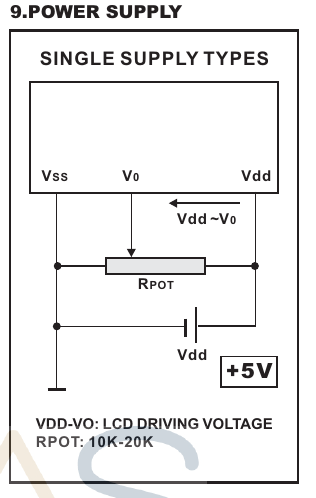
\includegraphics[width=0.3\textwidth]{img/LCD_Supply.png}
    \caption{Fig 1. : Alimentation et réglage du contraste de l'écran LCD}
    \label{fig:}
  \end{center}
\end{figure}


\section{Rôle du régulateur de tension}
Le régulateur de tension permet de convertir une tension délivrée par une pile 9 V en 5 V, ce qui est la tension acceptée par le PIC, le LCD et l'INA.


\section{Bits de configuration}

Conformément a ce qui avait été fait lors des TP d'électronique numérique, nous avons changé les bits de configuration suivants:\\

\begin{lstlisting}
FOSC  INTIO7
WDTEN OFF
LVP   OFF
\end{lstlisting}

Nous réglons l'horloge à 4Mhz à l'aide du registre \texttt{OSCCON} :\\

% Ok ici on a un bon tableau
% Le noindent est pour enlever l'indentation (sinon le tableau déborde dans l'autre sens
% Ici on utilise tabularx qui est une version améliorée de tabular
% |*{8}{C|} signifie qu'on crée 8 colonnes avec un bord (d'où le |) et dont le contenu est centré
\noindent
\begin{tabularx}{\textwidth}{|c|C|C|C|c|c|C|C|}
  \hline
  \multicolumn{8}{|>{\hsize=8\hsize}c|}{\texttt{OSCCON}}\\
  \hline
  % Ici on met le contenu des bits
  0 & 1 & 0 & 1 & 0 & 0 & 1 & 0\\
  \hline
  % Et ici les explications
  X 
  & \multicolumn{3}{>{\hsize=3\hsize}C|}{Horloge à 4Mhz} 
  & X & X 
  & \multicolumn{2}{>{\hsize=2\hsize}C|}{Utilisation de l'horloge interne}\\
  \hline
\end{tabularx}\\

Et on règle les interruptions:\\

\noindent
\begin{tabularx}{\textwidth}{|C|C|c|C|c|c|c|c|}
  \hline
  \multicolumn{8}{|>{\hsize=8\hsize}c|}{\texttt{INTCON}}\\
  \hline
  % Ici on met le contenu des bits
  1 & 1 & X & 1 & X & X & X & X\\
  \hline
  % Et ici les explications
  Activation des interruptions globales 
  & Activation des interruptions périphériques
  & X
  & Activation de l'interruption sur INT0
  & X & X & X & X\\
  \hline
\end{tabularx}\\\\

\noindent
\begin{tabularx}{\textwidth}{|C|C|c|c|c|c|c|c|}
  \hline
  \multicolumn{8}{|>{\hsize=8\hsize}c|}{\texttt{INTCON2}}\\
  \hline
  % Ici on met le contenu des bits
  1 & 0 & X & X & X & X & X & X\\
  \hline
  % Et ici les explications
  Désactivation des résistances de tirage &
  Interruption sur front descendant
  & X & X & X & X & X & X\\
  \hline
\end{tabularx}\\

\section{Programme en assembleur}
\subsection{Communication avec le LCD}
La partie du programme chargée de communiquer avec le LCD est clairement ce qu'il y a de plus technique dans le programme en assembleur. En effet, la datasheet du LCD impose un fonctionnement très précis pour les routines de calibration de l'écran et la communication entre l'écran et un microcontrôleur. De plus, la communication s'effectue sur plus de huits bits : il y a 8 bits associés à des commandes et 3 bits spéciaux qui permettent à l'écran de comprendre s'il est en mode lecture, écriture, etc. Les trois bits spéciaux sont RS (Register Select) et R/W (Read / Write) qui définissent le mode de communication actuel avec le pilote de l'écran, et E (Enable) qui valide une commande en passant à l'état bas. Tant que E est à sa valeur haute, les registres à l'entrée du LCD se chargent mais ne sont pas encore relevés par l'écran. Le front descendant va définir le moment où l'écran va relever les valeurs qu'on lui a transmises.
On est donc sensé envoyer 11 bits en paralèlle alors que nos registres n'en comportent que 8. Cela justifie la raison pour laquelle il fallait configurer l'écran pour fonctionner en instructions 4 bits. Nous avions vite deviné que c'était le cas car les pins DB0:3 n'étaient pas connectés sur le montage.

\paragraph{Dimensionnement des routines de temporisation}
Pour communiquer avec l'écran LCD, le plus important était d'avoir des routines de temporisations correctes. En effet, entre chaque commande envoyée à l'écran LCD, il faut attendre une durée minimale pour que la commande soit validée. Comme la plupart des commandes demandaient une attente de $ 38 \mu s $ . Nous avons donc créé une routine de temporisation software qui prend la valeur d'un registre UNIT\textunderscore WAIT et la décrémente jusqu'à atteindre la durée désirée. Pour nous assurer du bon fonctionnement de la routine de temporisation nous avons fait un programme qui tourne en boucle afin de générer un signal créneau sur une des pattes du microcontrôleur. Puis nous avons capté ce signal créneau au moyen de l'oscilloscope afin de vérifier que la routine de temporisation unitaire permettait bien d'introduire une attente supérieur à $ 38 \mu s $ .
Nous aurions pu utiliser l'horloge interne pour faire une routine de temporisation hardware, mais comme nous avions un temps limité pour améliorer le code et que les mesures à l'oscilloscope nous permettaient une précision raisonnable, nous avons laissé la routine en l'état.

Une fois cette routine de temporisation unitaire disponible, nous avons utilisé des boucles imbriquées pour introduire les temps d'attentes nécessaires aux différentes commandes. Il est bon de noter par exemple que la commande de calibraton de l'écran demande un temps d'attente de l'ordre de 40 millisecondes, ce qui impliquait au moins deux boucles imbriquées avec des compteurs sur huits bits pour pouvoir attendre suffisamment longtemps ( 0xFF = 256 et $256 * 40 \mu s  \neq 40 ms$ ).

Nous avons aussi fait une routine de temporisation encore plus importante pour le rafraichissement de l'écran. Il s'agissait de fixer ce qu'on appelle le framerate, à savoir combien d'affichage différents auront lieu par seconde. En effet, même avec 40 millisecondes d'attente, on affiche encore beaucoup trop de caractères différents par seconde, ce qui rend l'affichage illisible. C'est notamment le cas car les valeurs renvoyées par la cellule de pesée avaient tendance à osciller légèrement de $\pm 2 \times \frac{5}{1024}$ e de volts. Nous avons donc choisi de limiter l'affichage à environ 3 affichages par seconde.

\paragraph{Conception de la routine de calibration de l'écran}
La partie la plus hardue de la communication avec l'écran est de la calibrer, et de le faire correctement afin qu'il fonctionne bien en instructions sur 4 bits, autrement toutes les communications qui suivront ne feront que générer des effets inattendus. Le problème que nous avons rencontré est que la routine de calibration est dotée de plusieurs étapes avec des attentes précises et qu'on ne peut avoir d'information quant au fait que cela s'est bien passé. Il faut absolument terminer correctement la routine de calibration avant de voir apparaître un curseur.
Nous avons essayé par nous-mêmes d'appliquer la procédure décrite dans la datasheet, sans succès : le curseur n'apparaîssait pas.
Nous avons par la suite consulté M. Lambert qui nous a donné des conseils puis a fini par nous fournir le code de sa routine de calibration. En essayant de comparer son code au nôtre, nous n'avons dans un premier temps pas compris pourquoi notre routine ne fonctionnait pas car nous avions absolument le même déroulement et nous avions mesuré notre temps de temporisation et avions constaté qu'il était bien supérieur à ce qui était nécessaire.

Nous nous sommes finalement rendus compte que le montage conçu inversait la position des bits RS et R/W par rapport aux jeux d'instructions décris dans la datasheet. En échangeant ces deux bits dans toutes les commandes, nous avons eu immédiatement un écran calibré correctement et le message de test que nous avions codé pour constater le fonctionnement s'est affiché sans encombre.

\paragraph{Routines génériques pour la communication avec le LCD}

Une fois que nous nous sommes assurés que l'écran était correctement configuré, nous avons développé des fonctions utilitaires pour les opérations courantes :
\begin{itemize}
  \item VALIDATECMD charge le registre LATD avec la valeur stockée dans WREG, puis fait passer le bit E (Enable) à l'état bas et temporise pour qu'une commande envoyée soit acceptée par l'écran.
  \item WRITENUMBER affiche un chiffre de 0 à 9 en fonction de la valeur de WREG.
  \item WRITEG affiche le "g" des grammes
  \item Des routines comme TOLINE1 et CLEARDISPLAY permettent de déplacer le curseur sur l'écran.
\end{itemize}

En définitive nous nous sommes assez peu servis des routines TOLINE1 et autres fonctions permettant d'écrire sur plusieurs lignes. Durant nos tests nous avions réussi à nous en servir mais pour la fonctionnalité principale, nous n'en avons pas eu le besoin.

Pour afficher les chiffres nous avions d'abord conçu une table de correspondance avec un computed GOTO qui renverrait dans WREG le code sur 8 bits à afficher sur 4 bits en fonction de la valeur mise dans WREG. Cela fonctionnait dans un programme indépendant, en revanche, une fois intégré dans le programme général, la table ne fonctionnait plus. En effet, ajouter l'index au PCL envoyait le programme environ 200 lignes trop loin. C'est dû au fait que dans le programme indépenant, le faible nombre d'instructions faisaient qu'on pouvait compter les instructions sur uniquement 256 valeurs, alors que dans le programme général, le PCH intervient aussi lorsqu'il y a plus de 256 instructions. Nous nous sommes retrouvés avec un computed GOTO qui ne fonctionnait pas car cela impliquait aussi de gérer le most significant byte du program counter, en plus d'incrémenter le least significant byte (PCL). Comme cela n'est pas possible en une seule instruction et que cela impliquait de faire de la manipulation d'adresse mémoire un peu hasardeuse, nous avons décidé de procéder autrement.

\begin{lstlisting}
WRITENUMBER
    MOVWF NUMBER
    MOVLW b'01010011'
    CALL VALIDATECMD
    
    MOVLW b'01010000'
    IORWF NUMBER, 0
    CALL VALIDATECMD
    
    RETURN	    
\end{lstlisting}

La fonction WRITENUMBER par du constat très simple que les 4 bits de poids forts des caractères numériques sont toujours les mêmes. Par conséquent, la première moitié de l'instruction n'a jamais besoin d'être modifiée. En ce qui concerne les bits de poids faible, on part de "0000" pour le 0 et on compte en binaire jusqu'à "1001" pour 9. Il suffisait donc de faire un OU logique de la valeur du chiffre à afficher avec les bits E RS et R/W nécessaires pour envoyer le reste du code du caractère.

\subsection{Acquisition des valeurs en provenance du CAN}

Le CAN (convertisseur Analogique-Numérique) du PIC récupère le signal de sortie de l'ampli, qui est sur 5 V. Nous avons décidé de capter les valeurs sur 10 bits même si cela complique les calculs par rapport au mode 8 bits qui existe aussi. La raison pour laquelle nous avons choisi ce mode est que sur 8 bits, les 5 volts de dynamique seront répartis sur 256 bits soit des $\frac{5}{256}$ de Volt, alors que 10 bits permettent d'obtenir des $\frac{5}{1024}$ de Volt. Comme à charge pleine, soit 1 Kg, le signal de la cellule de pesée renvoie 5 Volts, on avait donc $\frac{1}{1024}$ e de Kg, ce qui est proche du gramme alors que la numérisation sur 8 bits faisait des pas d'environ 4g, ce qui correspond à une erreur potentielle de $\pm 4$g si le CAN utilise la méthode de la troncature pour la numérisation, ou $\pm 2$g pour la méthode de l'arrondi. Comme l'objectif d'une balance est d'offrir la meilleur précision, nous avons donc décidé d'utiliser l'acquisition sur 10 bits.

\paragraph{Récupération des valeurs numérisées}
Nous avons réutilisé le code réalisé en TP d'électronique numérique. Rien n'a été changé ou presque. 
Il y a une boucle de polling qui vérifie à chaque tick horloge si l'acquisition est terminée et, quand elle l'est, copie les valeurs dans les registres prévus à cet effet. \\
\begin{lstlisting}
LAUNCH
    BSF ADCON0,GO
    
POLL
    BTFSC ADCON0,GO
    BRA POLL
    
    ; If a new value has been captured, move the result in global vars
    MOVFF ADRESH, RESULTHI
    MOVFF ADRESL, RESULTLO
    
    RETURN 
\end{lstlisting}

Dans un premier temps nous avons testé l'acquisition avec la routine WRITECHAR qui affiche les caractères correspondant au code passé dans WREG. Nous ne relèvions que les 8 bits de poids faibles de la valeur que nous envoyions tels quels à la routine WRITECHAR. Cela nous a permis de constater que les variations de 1g changeaient bel et bien la valeur captée en temps réel.

\paragraph{Interruption physique}
Pour la fonctionnalité associée à l'interrupteur, nous avons aussi réutilisé telle quelle le code du TP. Nous avons fait une interruption qui affichait le caractère "7" quand on appuie sur le bouton pour constater son bon fonctionnement. Une fois le fonctionnemment établi, nous avons remplacer l'affichage par la routine de tare.

\section{Application de la tare}

Une tare peut être prise lors de l'appui sur le bouton. Celui-ci est relié à une pin capable de déclencher une interruption matérielle pour exécuter une routine.\\

\begin{lstlisting}
HIGH_ISR
    ; Reinitialise le bit dinterruption
    BCF INTCON, 1
    CALL TARE
    RETFIE  FAST
\end{lstlisting}

La routine de tare prend une mesure de l'entrée analogique et enregistre la valeur brute dans un registre mémoire.\\

\begin{lstlisting}
TARE
    CALL ACQUISITION
    MOVFF RESULTLO, DEAD_WEIGHTLO
    MOVFF RESULTHI, DEAD_WEIGHTHI
    RETURN
\end{lstlisting}

Cette valeur sera soustraite à la valeur mesurée avant conversion et affichage du poids.\\

\begin{lstlisting}
SHOWACQ
    CALL CLEARDISPLAY
    CALL ACQUISITION      
    MOVF DEAD_WEIGHTLO, 0		   
    SUBWF RESULTLO, 1
    BTFSS STATUS, 0		          
    INCFSZ DEAD_WEIGHTHI, 0	   
    SUBWF RESULTHI, 1		        
    BN NEG_VALUE		    
    
\end{lstlisting}

Pour que la tare soit correcte, il faut bien opérer une soustraction sur deux octets, en commençant par l'octet de poids faible et en faisant remonter une éventuelle retenue à la valeur qu'on soustrait à l'octet de poids fort. 
On peut noter que la deuxième partie de la soustraction n'est pas réalisée si l'octet de poids fort est déjà égal à zéro.

Compte tenu qu'un poids négatif n'a pas de sens au niveau physique, nous choisissons de bloquer la valeur à un minimum de 0g.


\section{Application d'un coefficient correcteur}

La tension de sortie de la cellule de pesée est linéaire. À l'aide de différents poids, nous avons mesuré et placé sur un graphe les valeurs retournées par le CAN. À ce graphe, nous avons rajouté les valeurs que nous attendions (500 pour 500 grammes par exemple). On peut rapidement voir, à première vue, que la pente provenant du CAN doit être corrigée pour obtenir la même pente que le poids réel. Pour approximer la pente du CAN, nous avons calculé les pentes entre chaque segments puis nous avons fait la moyenne de ceux-ci. Nous avons supprimé une partie des dernières mesures, celles-ci paraissant fausses.\\

\begin{tikzpicture}
\begin{axis}
\addplot table [x=Weight, y=CAN output, col sep=comma] {../values.csv};
\addplot table [x=Weight, y=Weight, col sep=comma] {../values.csv};
\end{axis}
\end{tikzpicture}

Une fois la pente trouvée, nous avons pu calculer un coefficient correcteur à appliquer sur la valeur du CAN après suppression de la tare. Pour vérifier notre coefficient, nous avons calculé les valeurs corrigées. On peut observer une différence de maximum $\pm{2}$ grammes.\\

Comme nous ne pouvons pas multiplier par un nombre décimal en assembleur, nous devons multiplier à l'aide d'une fraction qui s'approche le plus possible du coefficient correcteur. En assembleur, pour multiplier par une fraction, il faut multiplier par le numérateur puis faire une division euclidienne par le dénominateur. Comme on multiplie par le numérateur, il faut veiller à ne pas utiliser de valeurs trop élevées pour que la valeur maximum ne déborde pas au-delà des 2 octets disponibles.\\

Nous avons calculé un coefficient correcteur de 1,07954. En arrondissant à 1,08, nous pouvons effectuer la conversion à l'aide d'une fraction $\frac{27}{25}$, ce qui nous permet de rester dans la gamme des valeurs disponibles ($1023 * 27 = 27621$)\\

\section{Problèmes rencontrés}

Lors du premier branchement de la cellule de pesée sur l'oscilloscope, nous n'arrivions pas à observer un changement de tension significatif. Nous avons donc rapidement monté la cellule de pesée sur un support permettant de la manipuler sans la maintenir gauchement sur un bord de table.\\

Une fois la cellule montée sur le support, nous avons pu aisément observer la variation de tension en fonction de la variation de poids et nous avons pu commencer à calculer le gain nécessaire.

Cependant, la cellule de pesée avait bien un comportement linéaire mais uniquement à plus de 60g sur le plateau. Au-dessus de 60g, chaque variation de tension apparaissait sur l'oscilloscope, même en rajoutant moins de 10g. En revanche, en-dessous de 60g, la cellule de pesée ne sortait aucune variation de tension. C'est la raison d'origine pour laquelle nous avions décidé de fixer la jauge sur un support : nous cherchions à avoir un montage mécanique plus stable pour arriver à détecter les petites variation de poids. En effet, les mesures des valeurs renvoyées par la cellule de pesée tenue à la main faisaient ressortir le même problème.

Nous avons donc fini par en parler avec M. Lambert pour comprendre d'où venait le problème, notamment parce que nous soupçonnions une cellule de pesée défectueuse.
En montant les câbles de la cellule de pesée à l'envers, nous avons réussi à obtenir des mesures qui saturent à 5 mV lorsque la cellule de pesée ne porte aucun poids, et qui descend linéairement avec le poids qu'on lui ajoute. Nous avons pu constater que la dynamique de la cellule de pesée était tronquée car son zéro était décalé : avec le montage à l'envers, on voyait les variations pour les plus petits poids mais elle finissait par saturer bien plus rapidement que 0mV à 1Kg. Nous avons conclu que la jauge de contrainte devait avoir été déformée et donc avoir un décalage de sa valeur à vide. Il aurait été possible de s'en servir sur une dynamique complète à condition de décaler la valeur référence, mais compte tenu que la carte n'avait pas été conçue pour avoir une référence basse différente pour l'INA et pour le PIC, nous avons choisi plus simplement de changer de cellule de pesée.
Le changement a aussi confirmé le défaut de la précédente cellule : tous nos défaut de mesure ont disparu instantanément, que ce soit avec la cellule de pesée seule ou montée sur son support.
\end{document}
